%&"../net"
\endofdump
\tikzexternalize[prefix=cache/]{lab05}
\usepackage{gbt7714}
% https://shimo.im/docs/xJTTRDH6YrkcvvTG/read
\begin{document}
    \title{Write SDN Controller}
    \maketitle
    \tableofcontents
    \vfill
    Ryu provides software components with well defined API's that make it easy for developers to create new network management and control applications.
    \vfill
    \clearpage
    \section{建立网络}
    Set up the following network first:
    
    \hfill
    \begin{tikzpicture}
    \tikzstyle{host}=[draw]
    \tikzstyle{switch}=[draw]
    \tikzstyle{connection}=[]
    \tikzstyle{constr}=[right,font=\ttfamily\small]
    
\node (h1) [host] at (-0.5,0.5) {h1};
\node (s1) [switch] at (1.5,0.5) {s1};
\node (s3) [switch] at (3,2) {s3};
\node (s2) [switch] at (4.5,0.5) {s2};
\node (s4) [switch] at (3,-1) {s4};
\node (h2) [host] at (6.5,0.5) {h2};
\draw  (h1) edge (s1);
\draw  (s1) edge (s3);
\draw  (s3) edge (s2);
\draw  (s2) edge (s4);
\draw  (s4) edge (s1);
\draw  (s2) edge (h2);
\end{tikzpicture}

    使用给出的示例代码。
    \code{loopnet.py}

    \section{定时切换}
    Write an RYU controller that switches paths (h1-s1-s3-s2-h2 or h1-s1-s4-s2-h2) between h1 and h2 every 5 seconds. 

    查看修改流的定义函数。其中参数 \texttt{hard\_timeout} 用于定义丢弃流前的最大秒数。

    \codeseg{../ryu/ryu/ofproto/ofproto\_v1\_3\_parser.py}{2703}{2710}
    
    参数 \texttt{flags} 可以被指定为 \texttt{OFPFF\_SEND\_FLOW\_REM},可以用于在丢弃流后发出事件用于相关处理。

    \begin{quotation}
    \textbf{Flow-Removed}: Inform the controller about the removal of a flow entry from a flow table. Flow-Removed messages are only sent for flow entries with the 
    \begin{center}
        \verb"OFPFF_SEND_FLOW_REM"
    \end{center} flag set. They are
generated as the result of a controller flow delete requests or the switch flow expiry process when one of the
flow timeout is exceeded (see 5.5).\cite{openflow13}
    \end{quotation}

    \codeseg{../ryu/ryu/ofproto/ofproto\_v1\_3.py}{371}{372}

    处理丢弃事件,RYU 源码给出了例子:

    \codeseg{../ryu/ryu/ofproto/ofproto\_v1\_3\_parser.py}{2377}{2402}

    \verb"datapath.id" 用于识别交换机,\verb"s1"对应1号,\verb"s2"对应2号,依次类推。

    \begin{figure}[H]
        \centering
        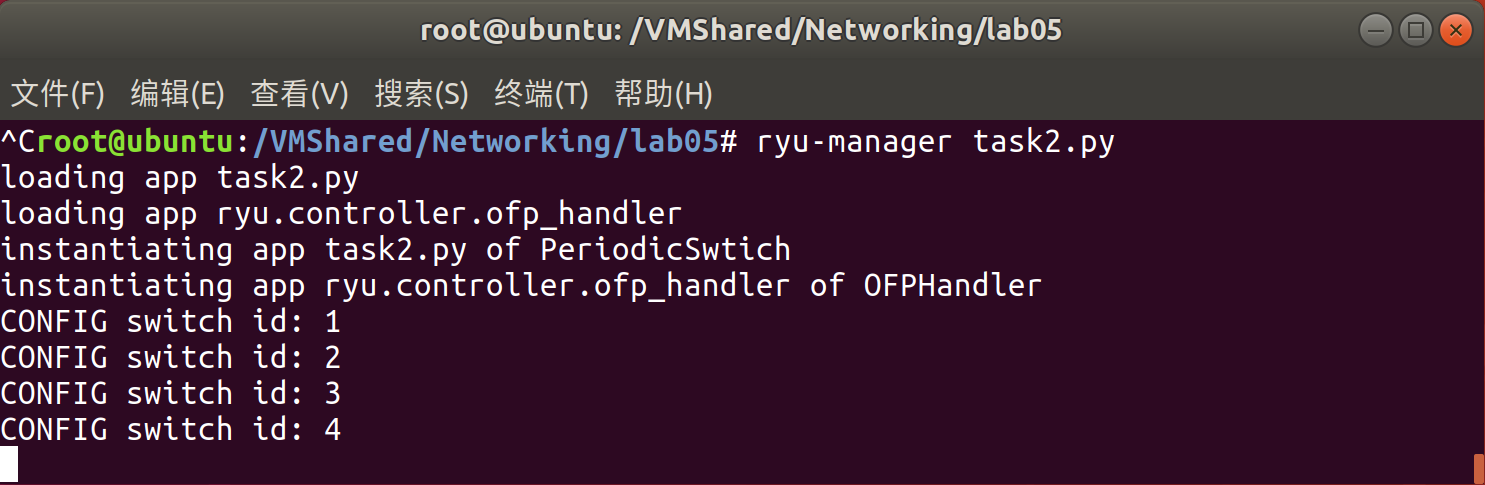
\includegraphics[width=0.6\linewidth]{idorder}
        \caption{交换机编号}\label{fig:idorder}
    \end{figure}

    使用下面的命令可以可视化地观察流信息\cite{gui},并启动控制器。
    \begin{lstlisting}[style=commandshell]
        ryu/ryu/app/gui_topology$ ryu-manager --observe-links gui_topology.py ../../../../lab05/task2.py\end{lstlisting}

    \begin{figure}[H]
        \centering
        \begin{minipage}{0.48\textwidth}
            \centering
            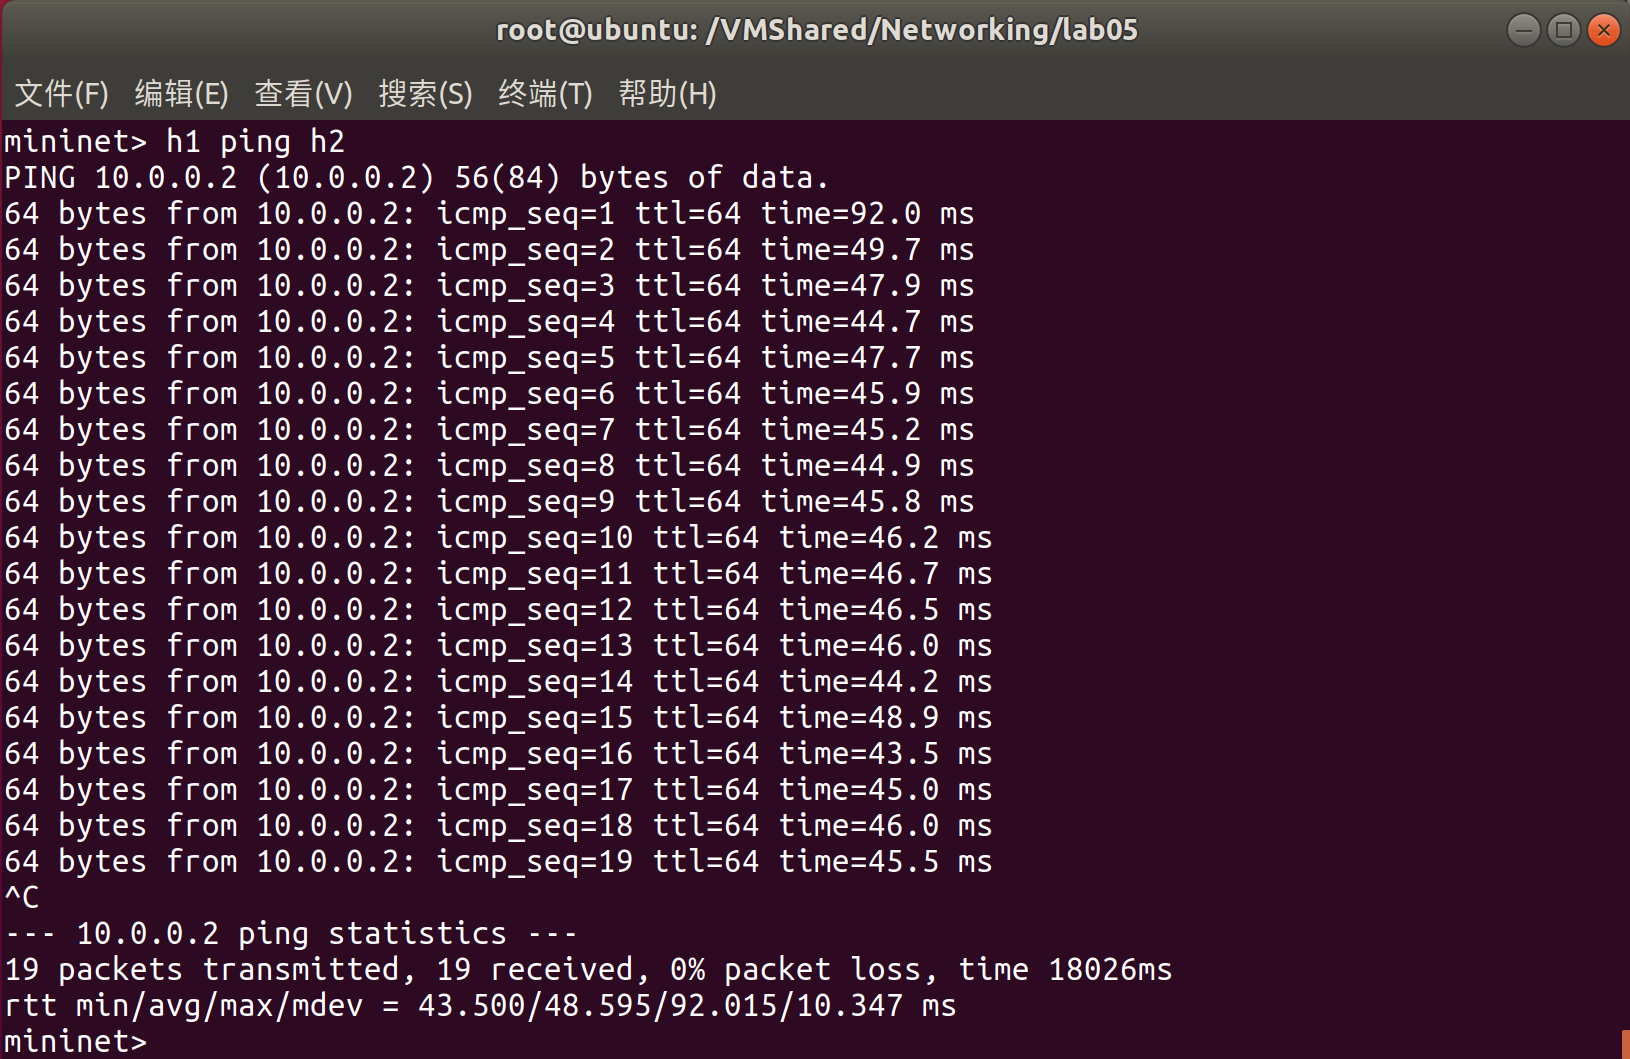
\includegraphics[width=\linewidth]{task2ping}
            \caption{测试连接}\label{fig:task2ping}
        \end{minipage}
        \begin{minipage}{0.48\textwidth}
            \centering
            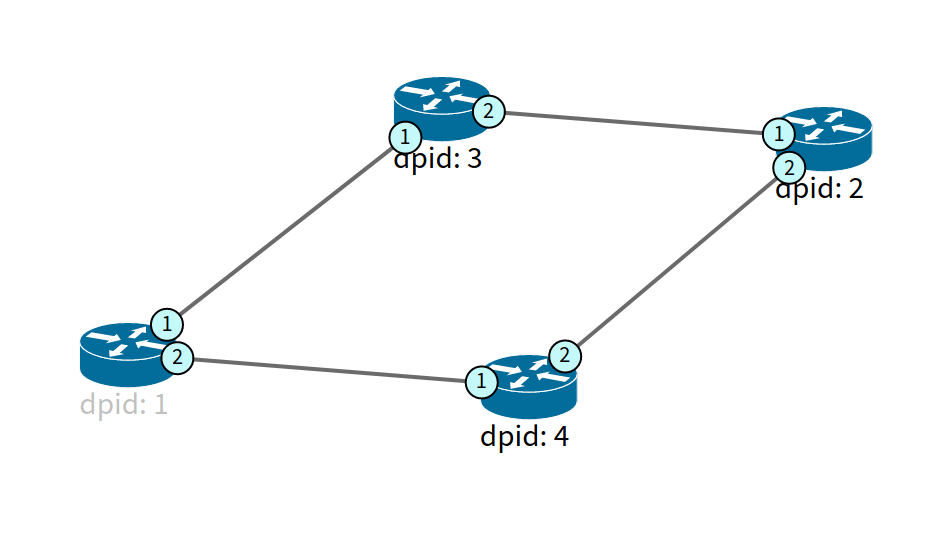
\includegraphics[width=\linewidth]{task2topo}
            \caption{\texttt{gui\_topology} 展示的拓扑结构}\label{fig:task2topo}
        \end{minipage}
    \end{figure}

    由图 \ref{fig:task2topo} 可见,可以通过定时切换 \verb"s1" 和 \verb"s2" 的输出端口,来达到切换链路的功能。切换为 \verb"3" $\rightarrow$ \verb"1" 采用上面的链路,切换为 \verb"3" $\rightarrow$ \verb"2" 采用下面的链路。在图 \ref{fig:task2ping} 中可见是能够 \verb"ping" 通的。相关代码见附录 \ref{sec:per5}。

    \section{}
    Write an RYU controller that uses both paths to forward packets from h1 to h2.

    \section{}
    Write an RYU controller that uses the first path (h1-s1-s3-s2-h2) for routing packets from h1 to h2 and uses the second path for backup. Specifically, when the first path experiences a link failure, the network should automatically switch to the second path without causing packet drop. (hint: consider using \verb"OFPGT_FF" (FF is short for ``fast failover'') to construct a group table)

    \bibliography{ref}

    \appendix

    \section{定时切换代码}\label{sec:per5}

    \code{task2.py}

\end{document}